\documentclass[10pt]{beamer}

\usepackage{settings}
\usepackage{minted}

\title{Cloud Computing}
\subtitle{Final Exam Exercise}
\date{\today}
\author[longname]{Giovanni Lucarelli}
\titlegraphic{\hfill
\includegraphics[height=1.3cm]{images/logo100_orizzontale.pdf}}

% add graphics path
\graphicspath{{../assets}}

\begin{document}

\maketitle

\begin{frame}{Goal}
  The goal is to assess and compare the performance of a cluster of two virtual nodes in different environment:
  \begin{itemize}
    \item Vitualbox
    \item Docker
  \end{itemize}
  \textbf{Benchmarks:}
  \begin{itemize}
    \item \texttt{hpcc}
    \item stress-ng
    \item sysbench
    \item IOZone
    \item iperf
  \end{itemize}
\end{frame}

\begin{frame}{(Virtual) Hardware Specification}
\textbf{\underline{Host Machine:}}
\begin{description}
  \item[CPU] Intel Core i7-8550U CPU @ 1.80GHz, \\4 Cores / 8 Threads
  \item[Memory] 8 GB
  \item[Disk] 256 GB SSD
  \item[OS] Ubuntu 24.04.2 LTS
\end{description}

\textbf{\underline{Cluster Nodes:}}
\begin{description}
  \item[CPU] 2 Cores
  \item[Memory] 2048 MB
  \item[Disk] 20 GB
  \item[OS] Ubuntu 22.04.5 live server (amd64)   
\end{description}
\end{frame}

\begin{frame}{High Performance Computing Challenge (HPCC)}
  \begin{description}
    \item[Computational:] \texttt{HPL}, \texttt{DGEMM}, \texttt{FFT}
    \item[Memory:] \texttt{STREAM}, \texttt{PTRANS}, \texttt{RandomAccess}
    \item[Communication:] \texttt{PingPong}, (\texttt{PTRANS})
  \end{description}
\end{frame}

\begin{frame}{HPCC: Computational Performance}
\begin{figure}
  \centering
  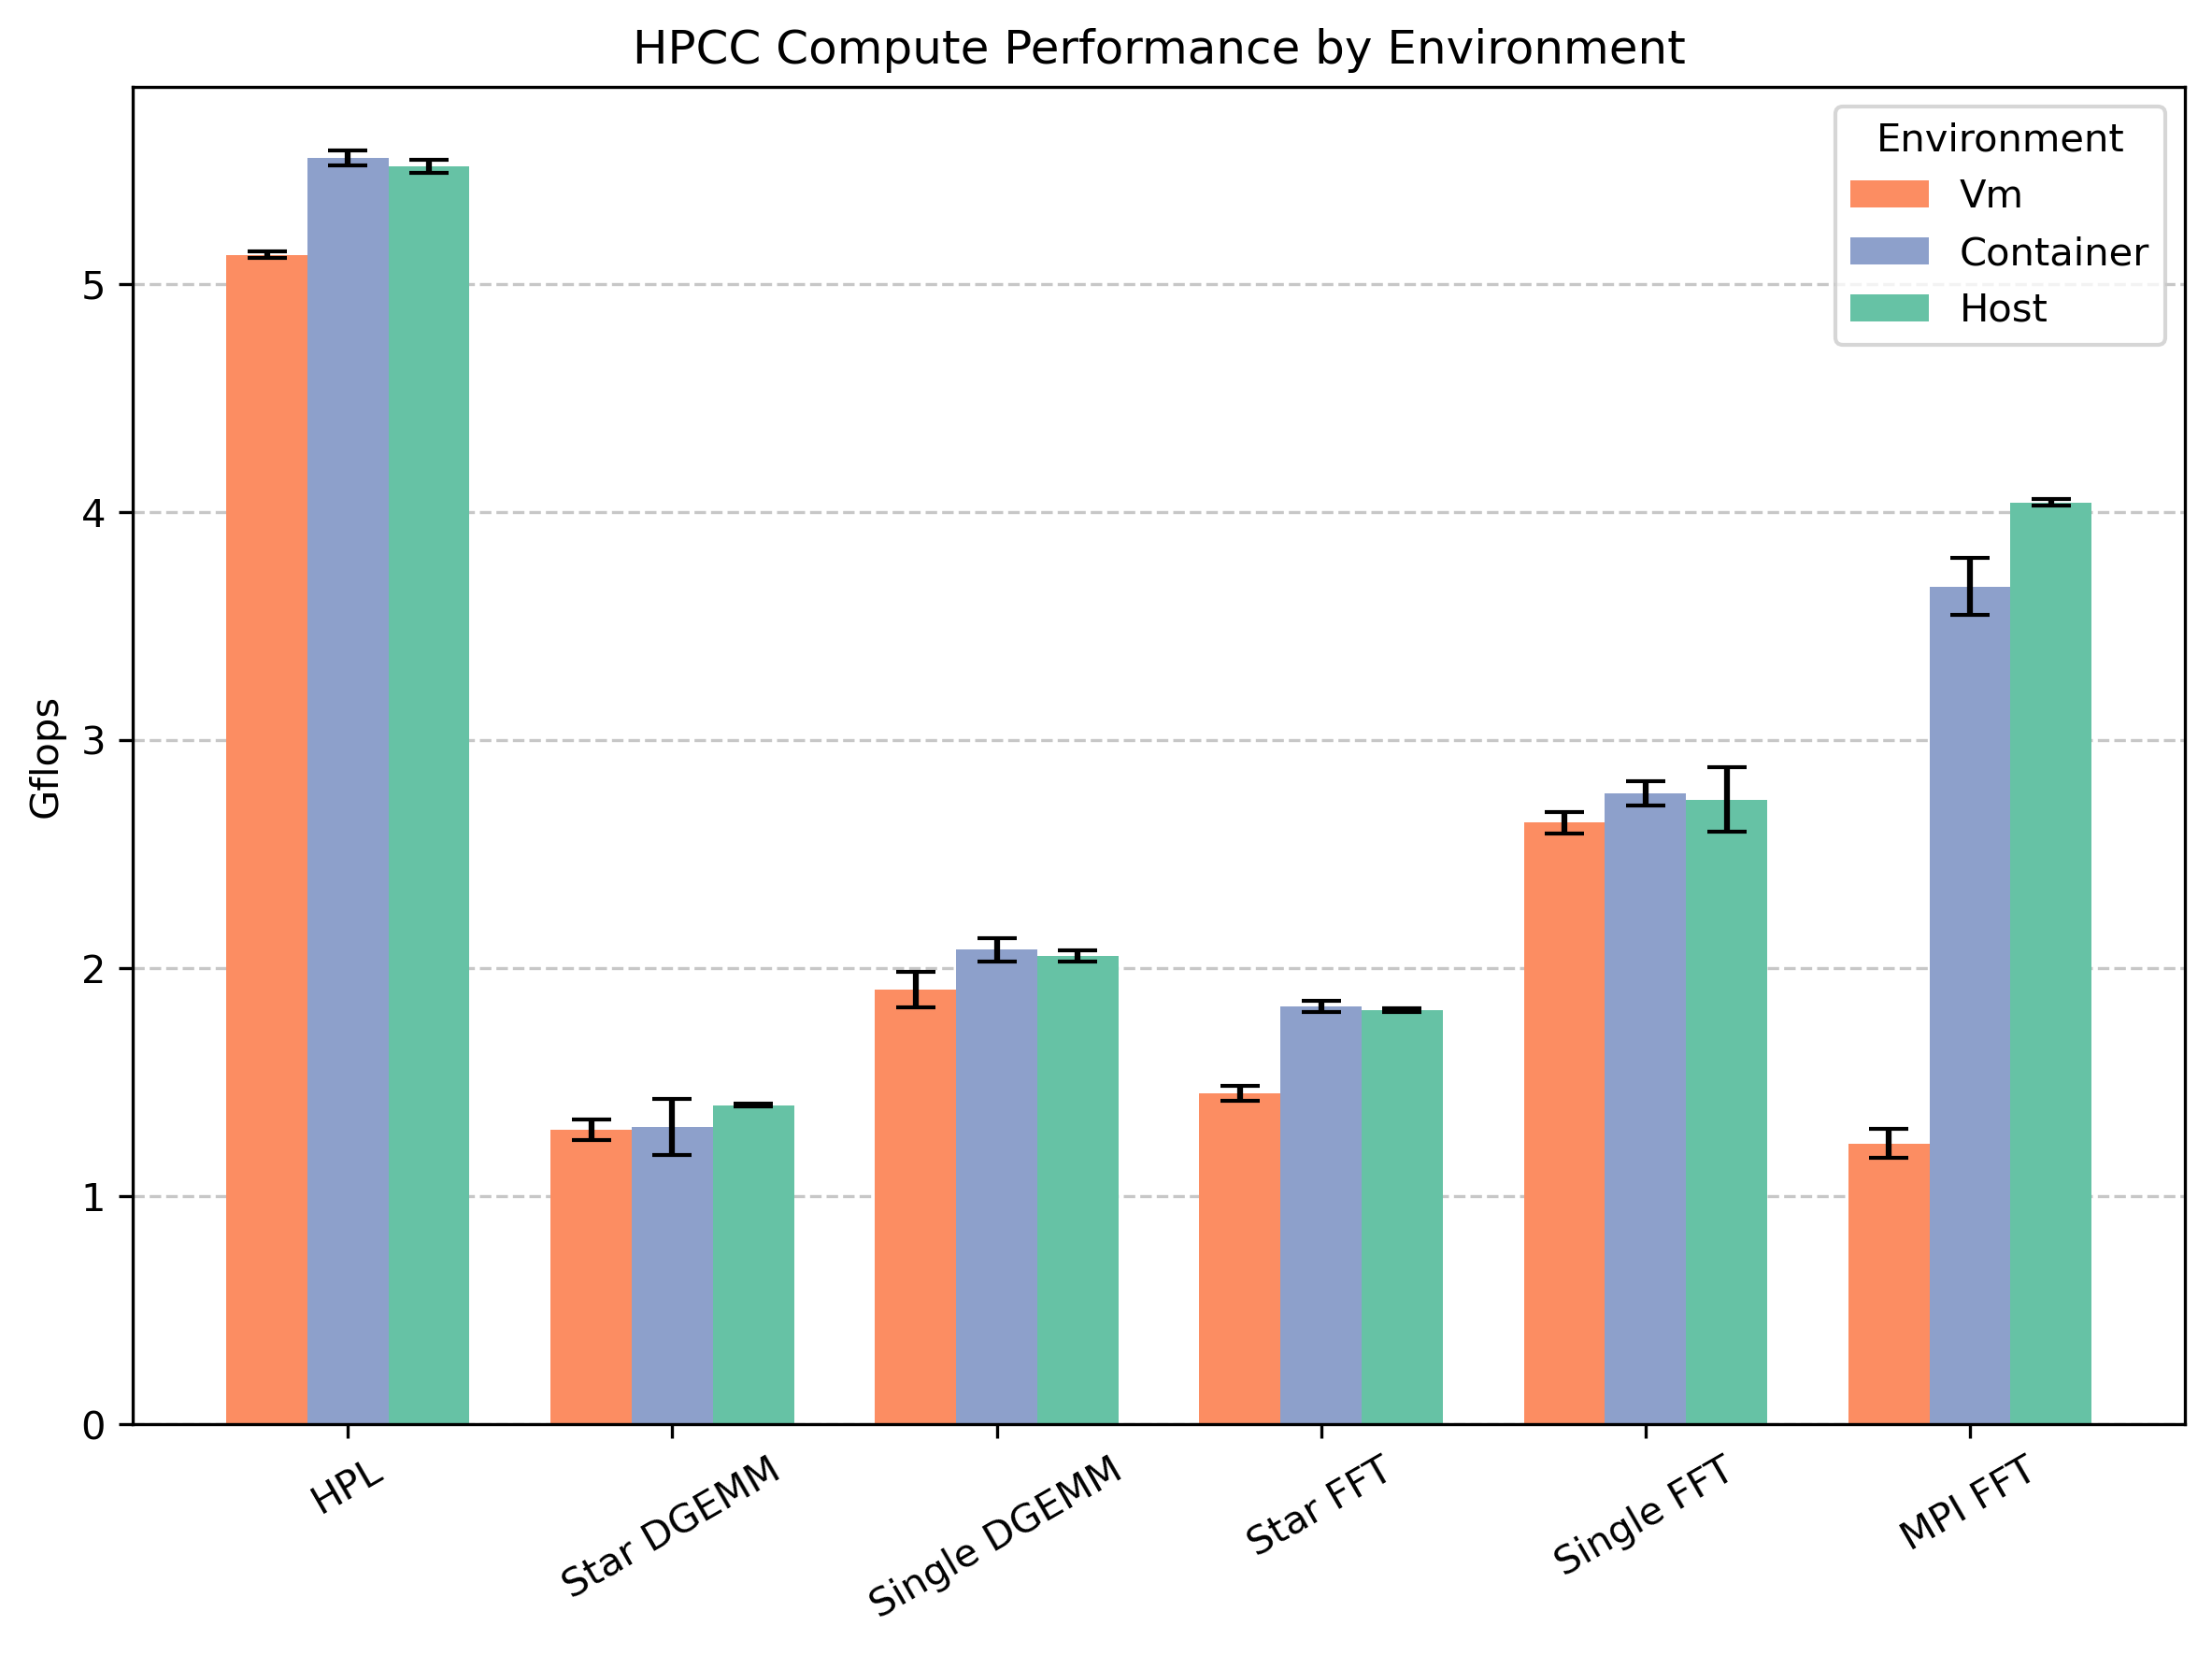
\includegraphics[width=0.8\textwidth]{hpcc_compute_performance.png}
\end{figure}

\end{frame}


\begin{frame}{HPCC: Memory Performance (1/3)}
  % TODO: plot

  \begin{table}[htbt]
  \centering
  \begin{tabular}{lccc}
  \toprule
  \textbf{Benchmark} & \textbf{VM} & \textbf{Container} & \textbf{Host} \\
  \midrule
  \textbf{SingleSTREAM (GB/s)} & & & \\
  Copy   & 22.30 ± 0.32 & 24.11 ± 0.20 & 23.44 ± 0.06 \\
  Scale  & 13.26 ± 0.19 & 14.23 ± 0.06 & 14.06 ± 0.12 \\
  Add    & 14.40 ± 0.24 & 15.38 ± 0.16 & 15.06 ± 0.14 \\
  Triad  & 14.44 ± 0.28 & 15.48 ± 0.13 & 15.22 ± 0.05 \\
  \midrule
  \textbf{StarSTREAM (GB/s)} & & & \\
  Copy   & 5.03 ± 0.03 & 5.41 ± 0.03 & 5.39 ± 0.02 \\
  Scale  & 3.34 ± 0.03 & 3.55 ± 0.01 & 3.56 ± 0.01 \\
  Add    & 3.75 ± 0.01 & 4.08 ± 0.02 & 4.07 ± 0.01 \\
  Triad  & 3.72 ± 0.04 & 4.02 ± 0.02 & 4.00 ± 0.02 \\
  \bottomrule
  \end{tabular}
  \end{table}

\end{frame}

\begin{frame}{HPCC: Memory Performance (2/3)}
  A comment about the nomial bandwidth of the memory
  
\end{frame}

\begin{frame}{HPCC: Memory Performance (3/3)}
  \begin{figure}
    \centering
    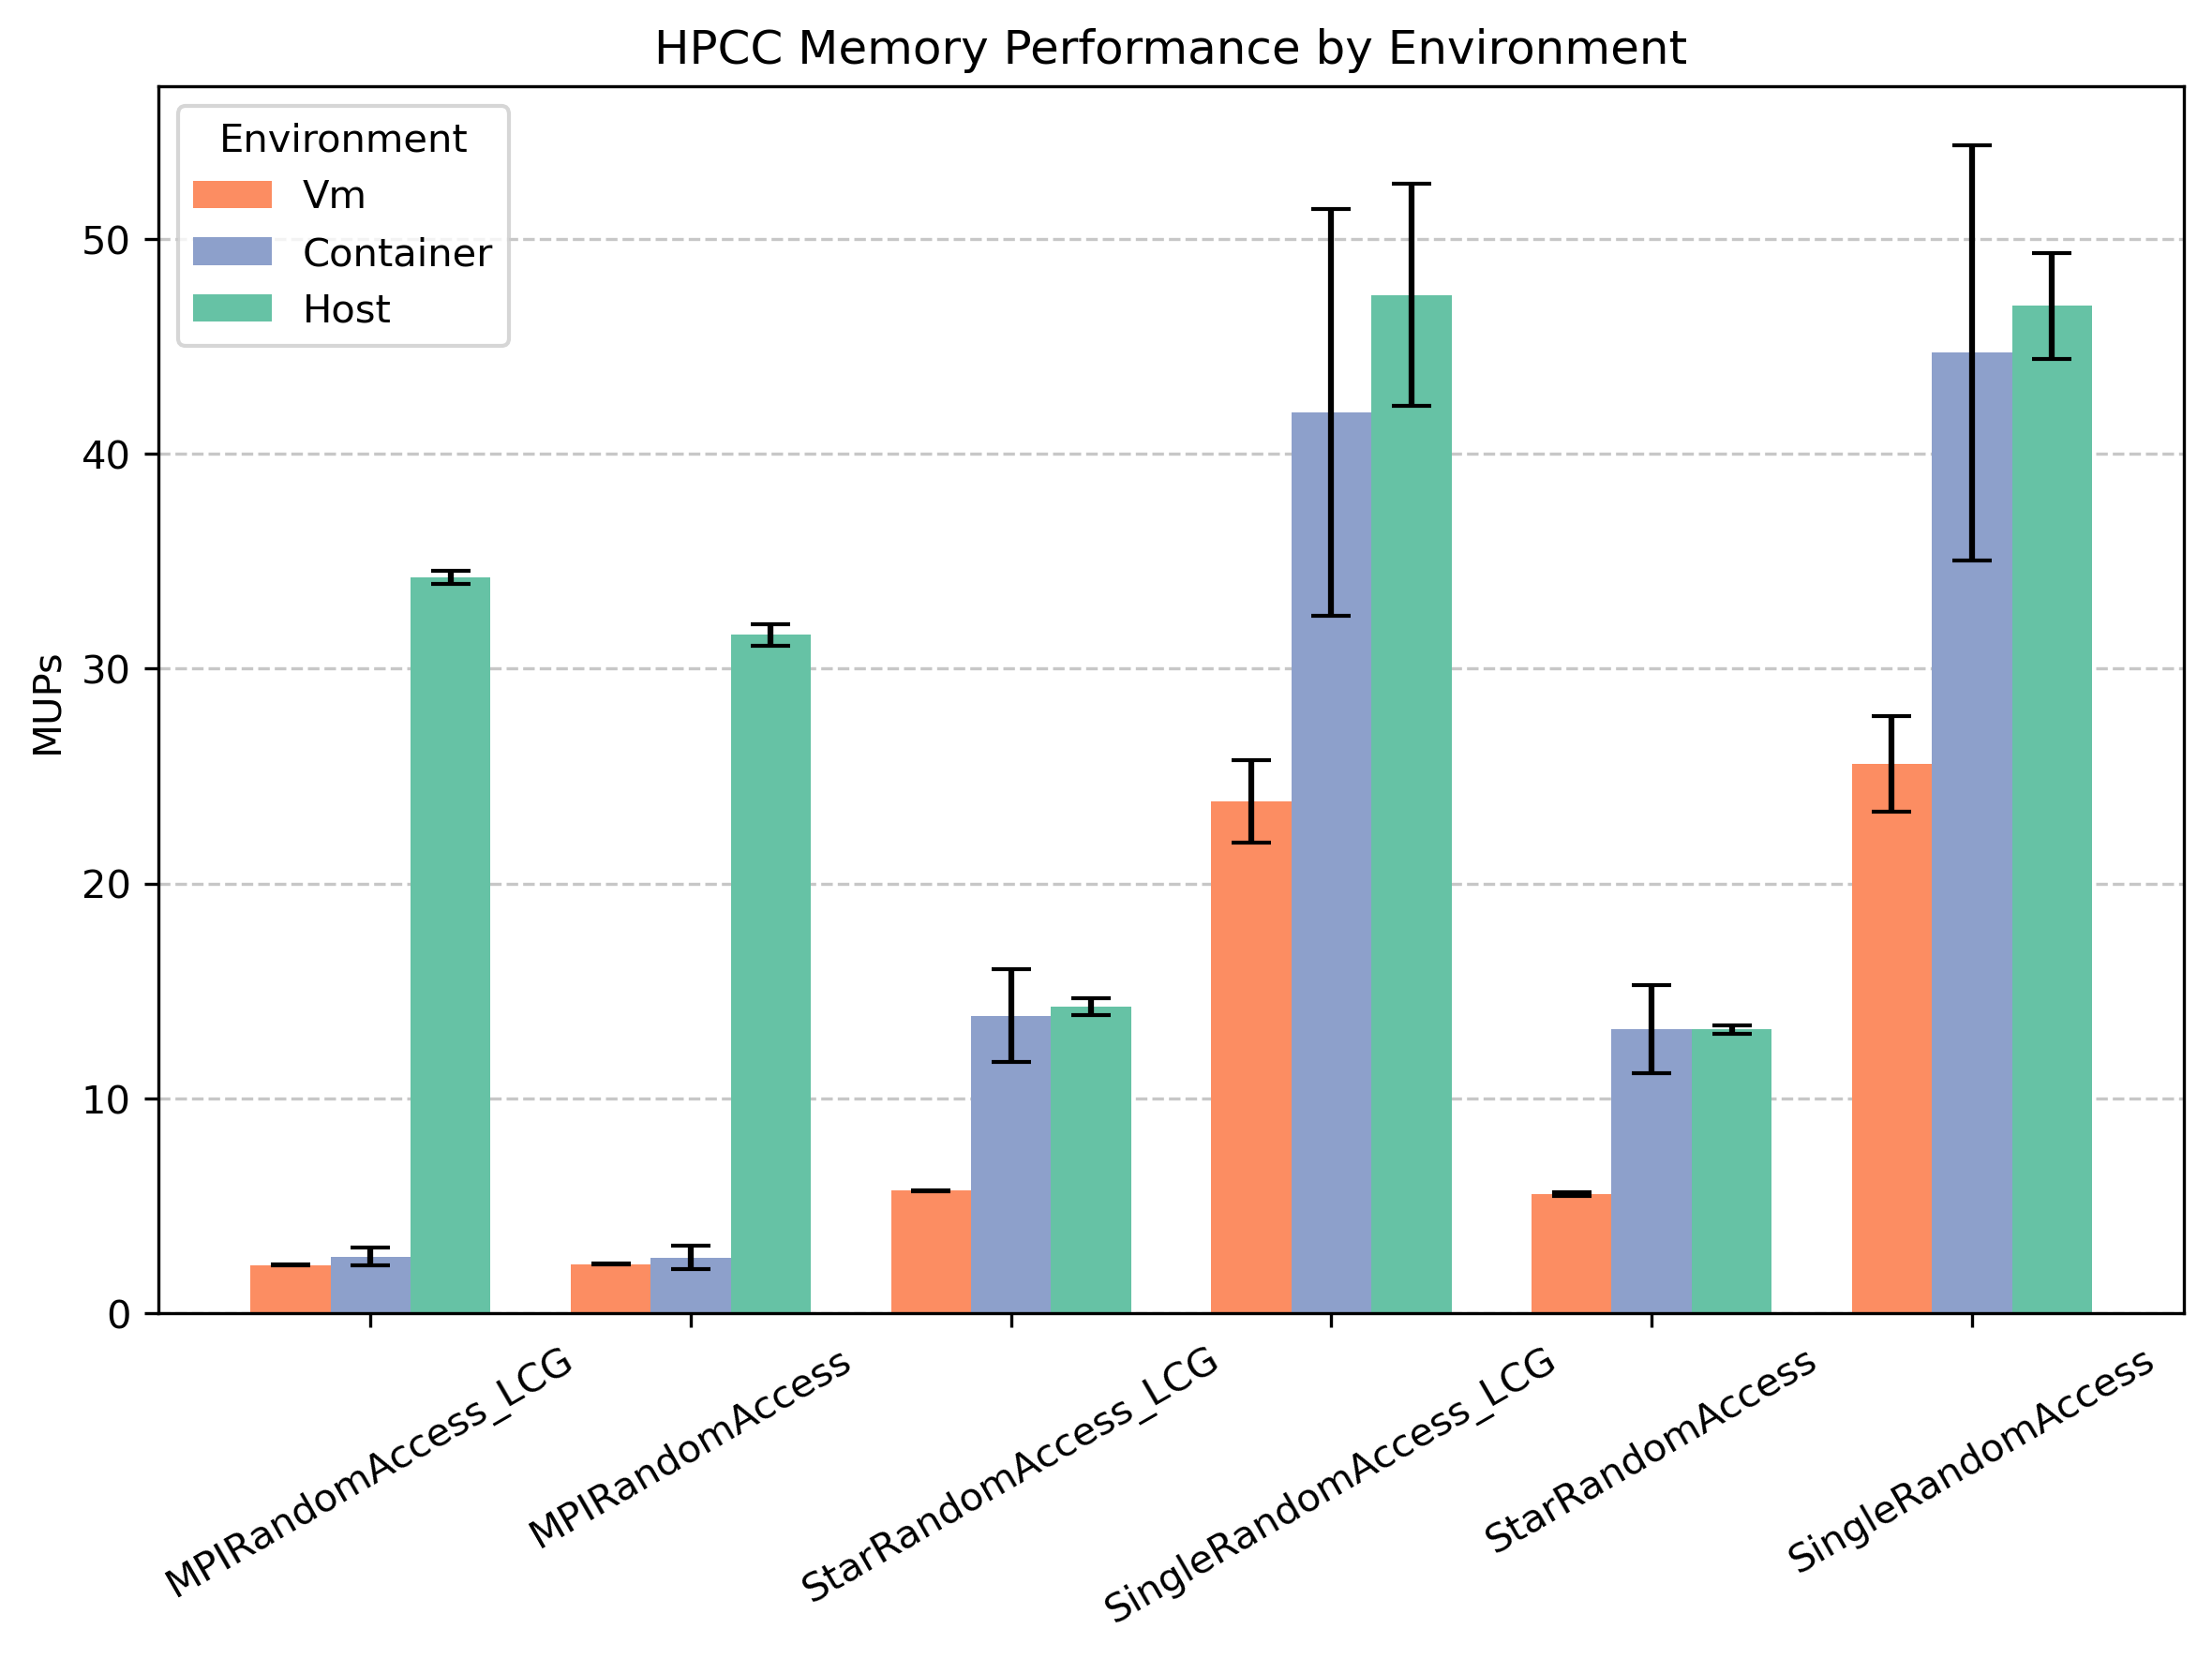
\includegraphics[width=0.8\textwidth]{hpcc_memory_performance.png}
  \end{figure}
\end{frame}

\begin{frame}{HPCC: Communication Performance}
  \begin{figure}
    \centering
    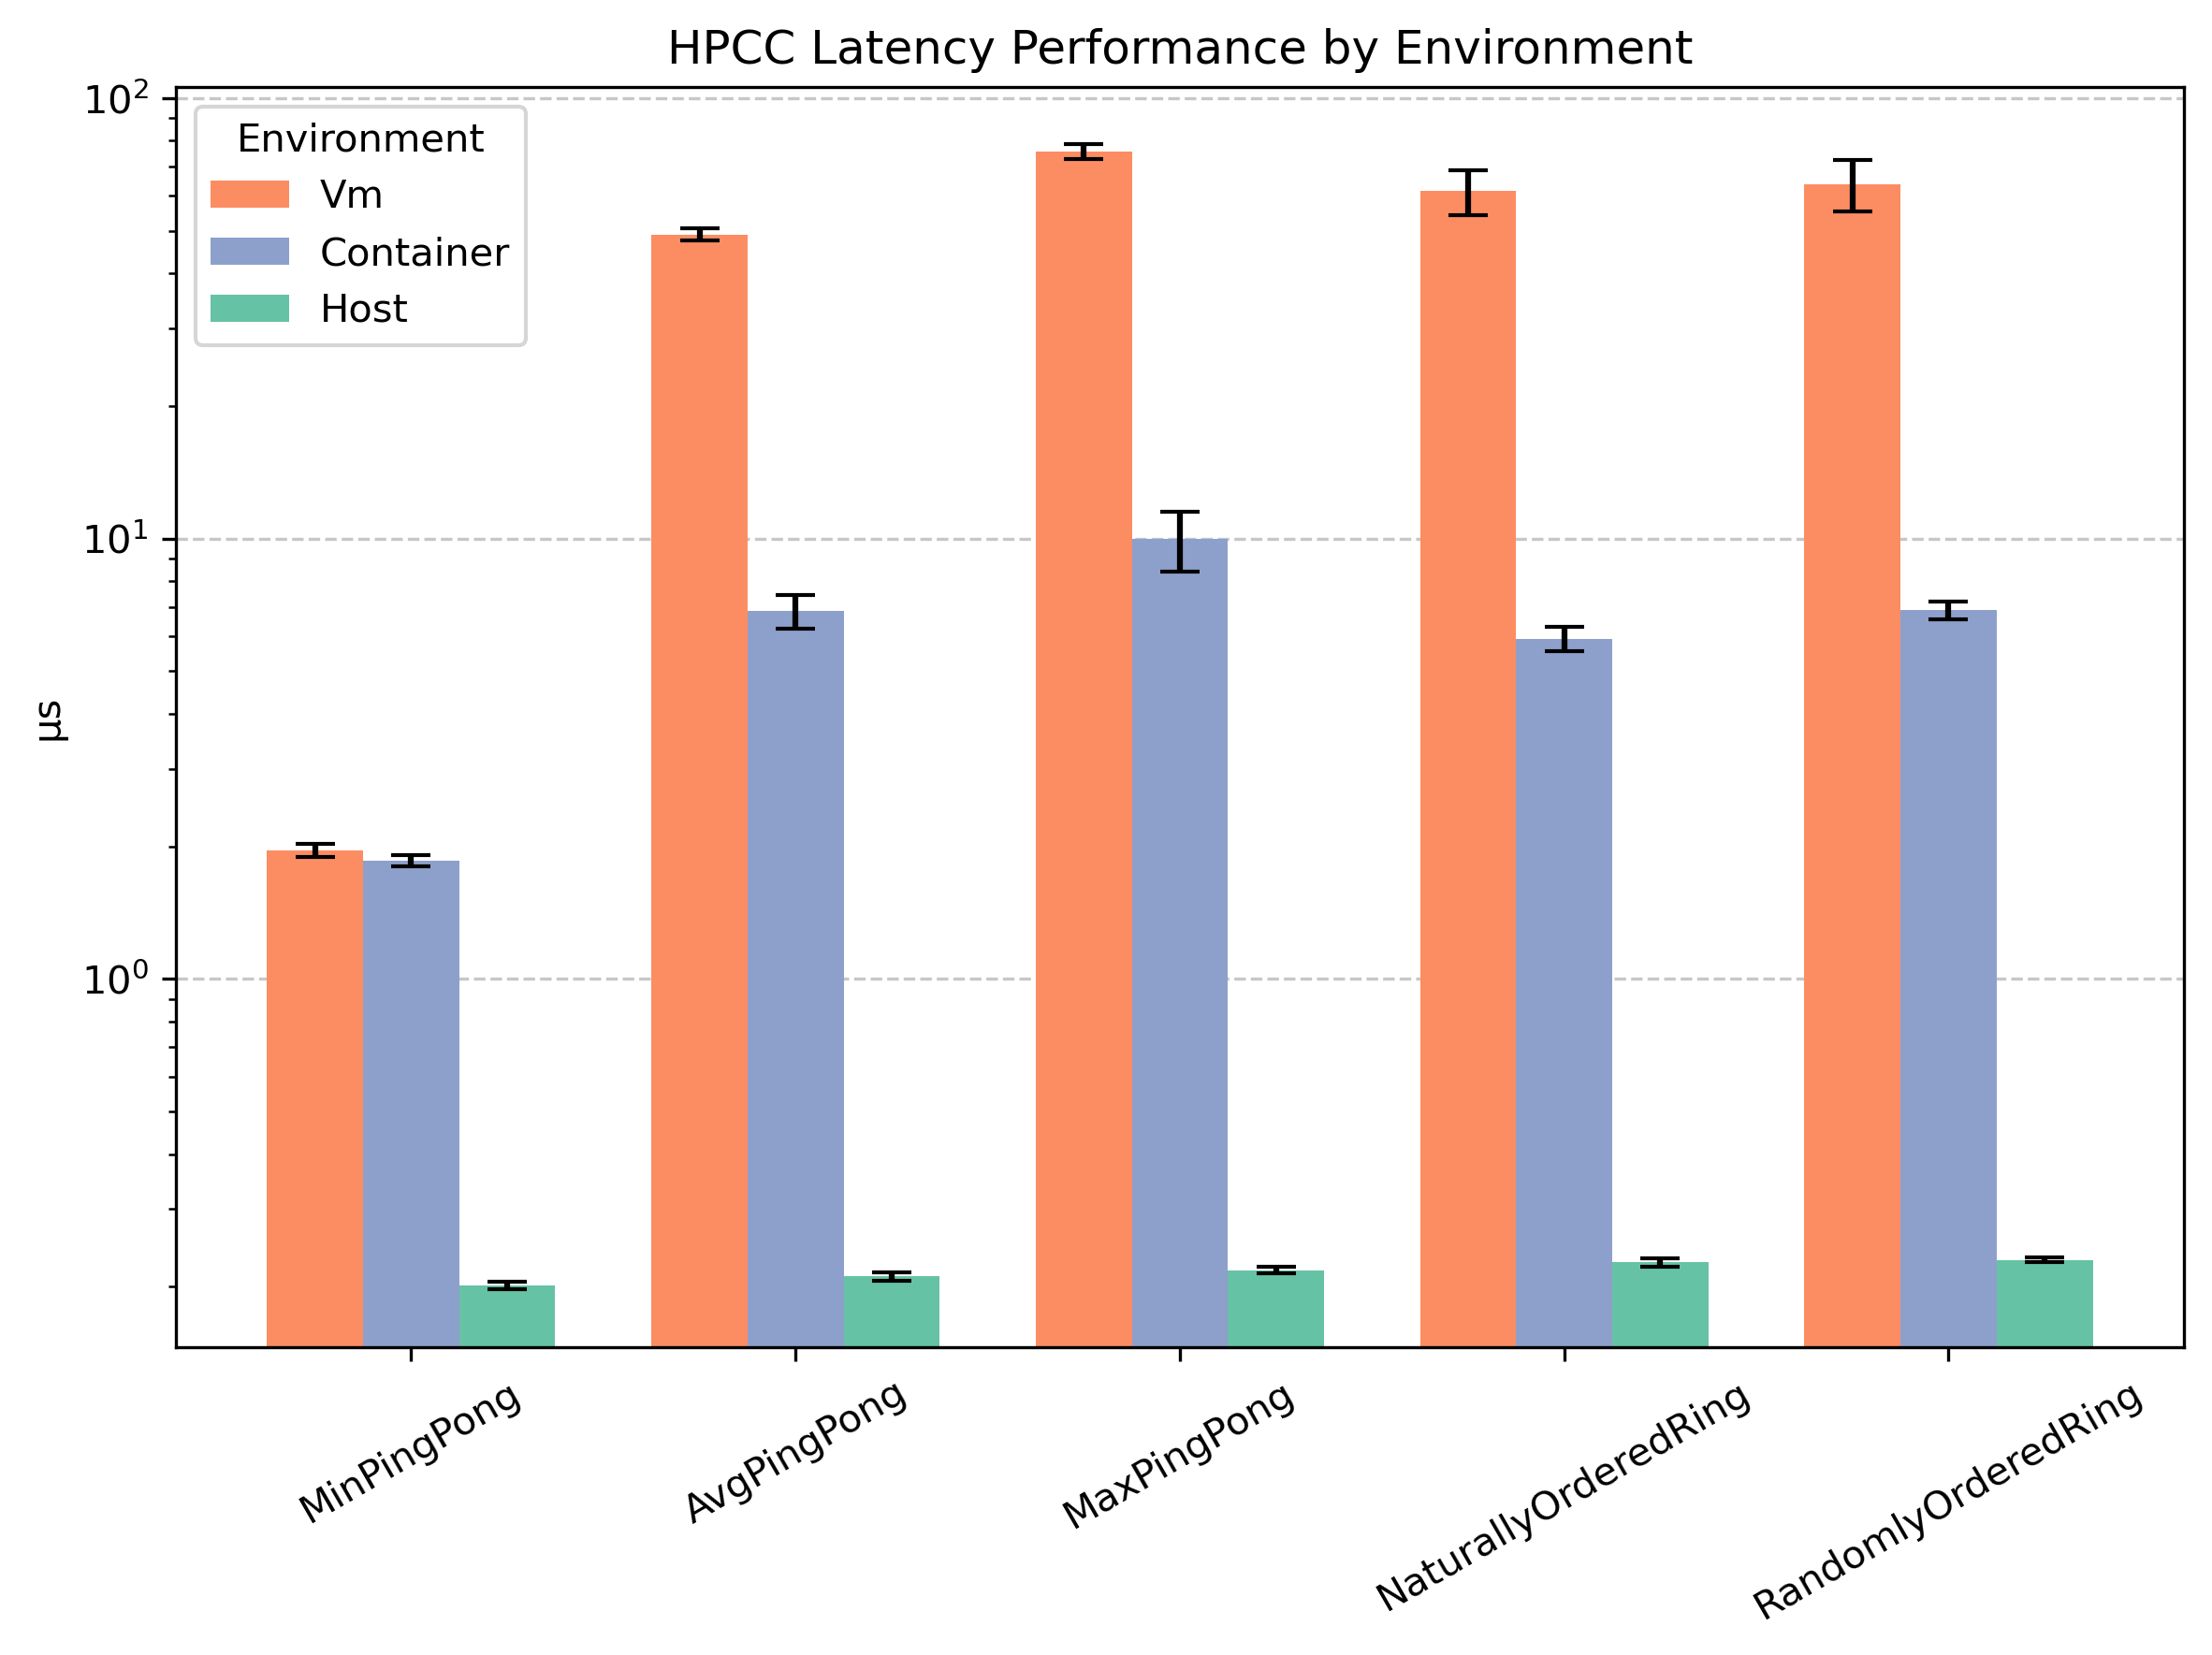
\includegraphics[width=0.8\textwidth]{hpcc_latency_performance.png}
  \end{figure}
\end{frame}

\begin{frame}{Stress-ng}
  % TODO: plot
\end{frame}


\begin{frame}{Sysbench}
  % TODO: plot
\end{frame}

\begin{frame}{IOZone: write local}
  \begin{figure}
    \centering
    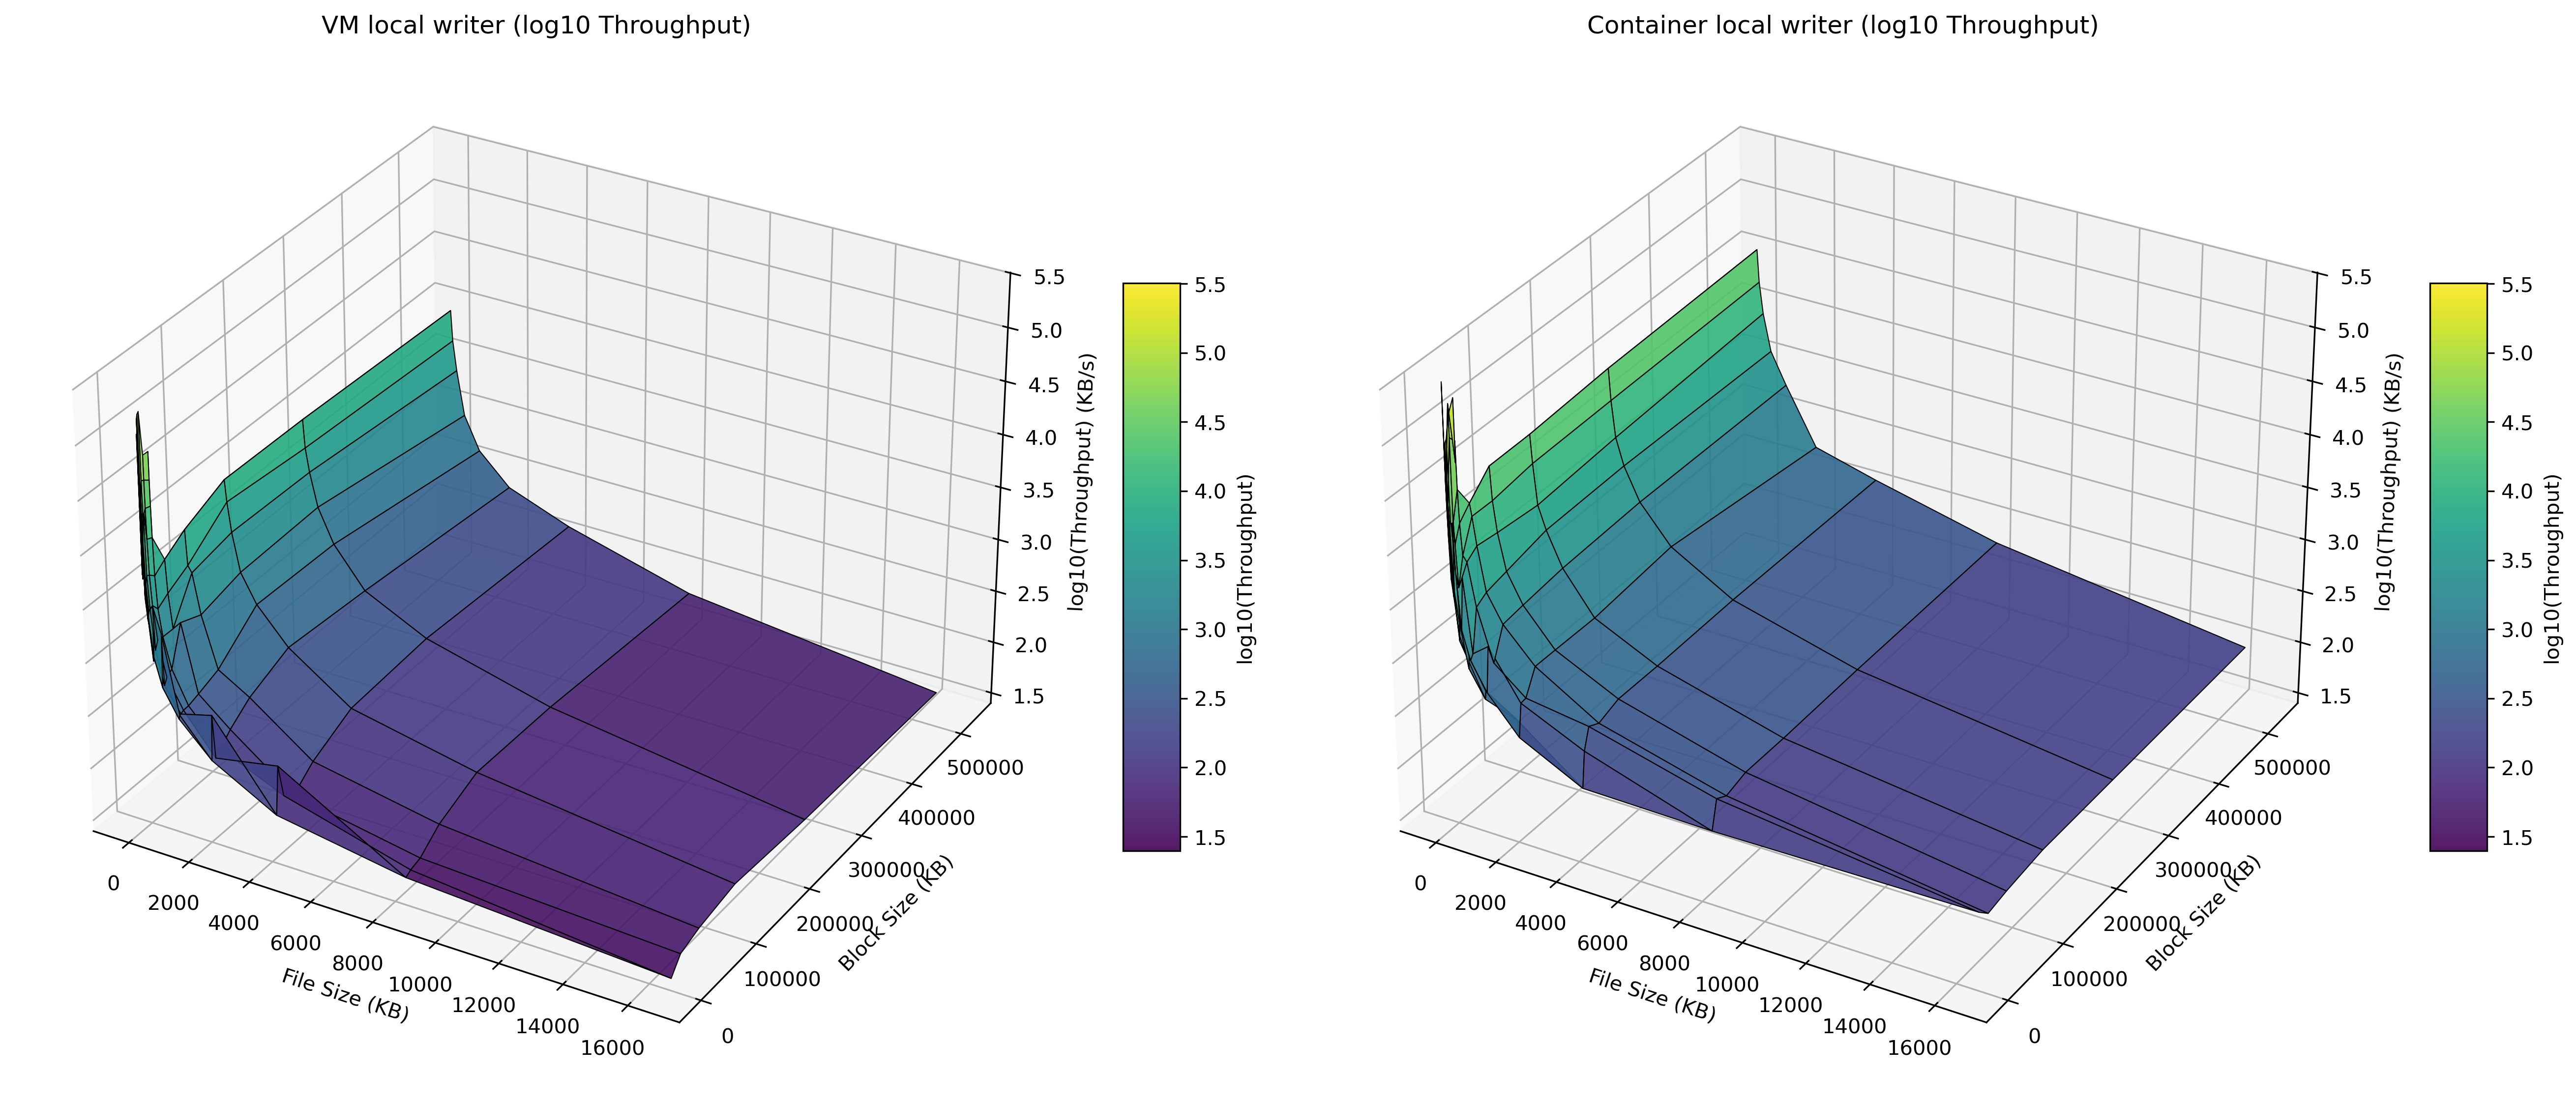
\includegraphics[width=\textwidth]{VM local writer_Container local writer_log_surfaces.png}
  \end{figure}
\end{frame}

\begin{frame}{IOZone: write shared}
  \begin{figure}
    \centering
    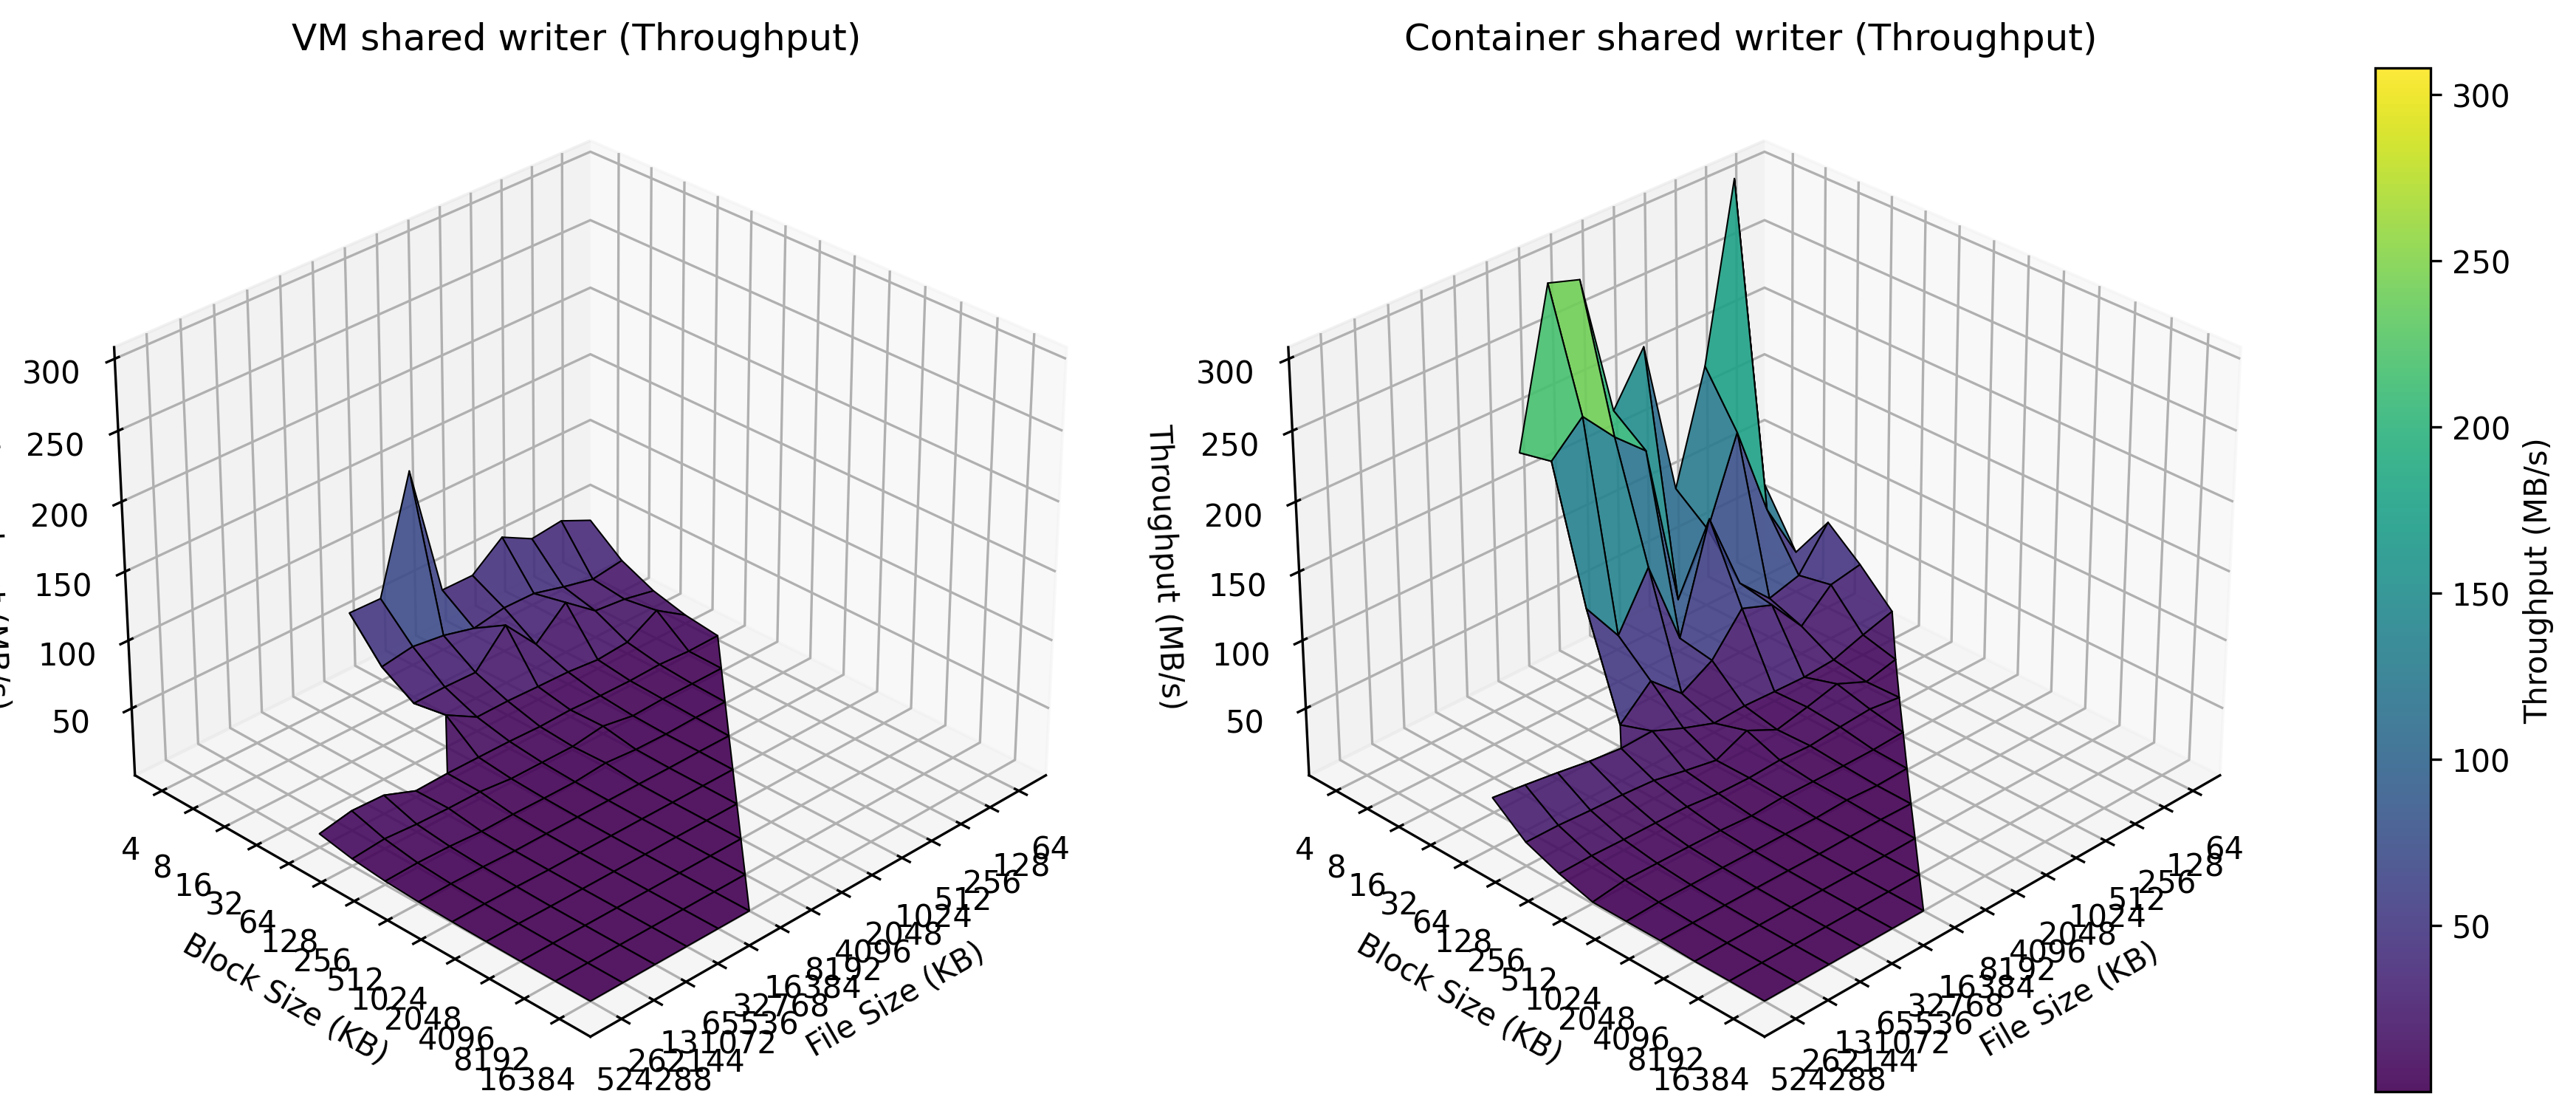
\includegraphics[width=\textwidth]{VM shared writer_Container shared writer_log_surfaces.png}
  \end{figure}
\end{frame}

\begin{frame}{IOZone: write}
  \begin{figure}
    \centering
    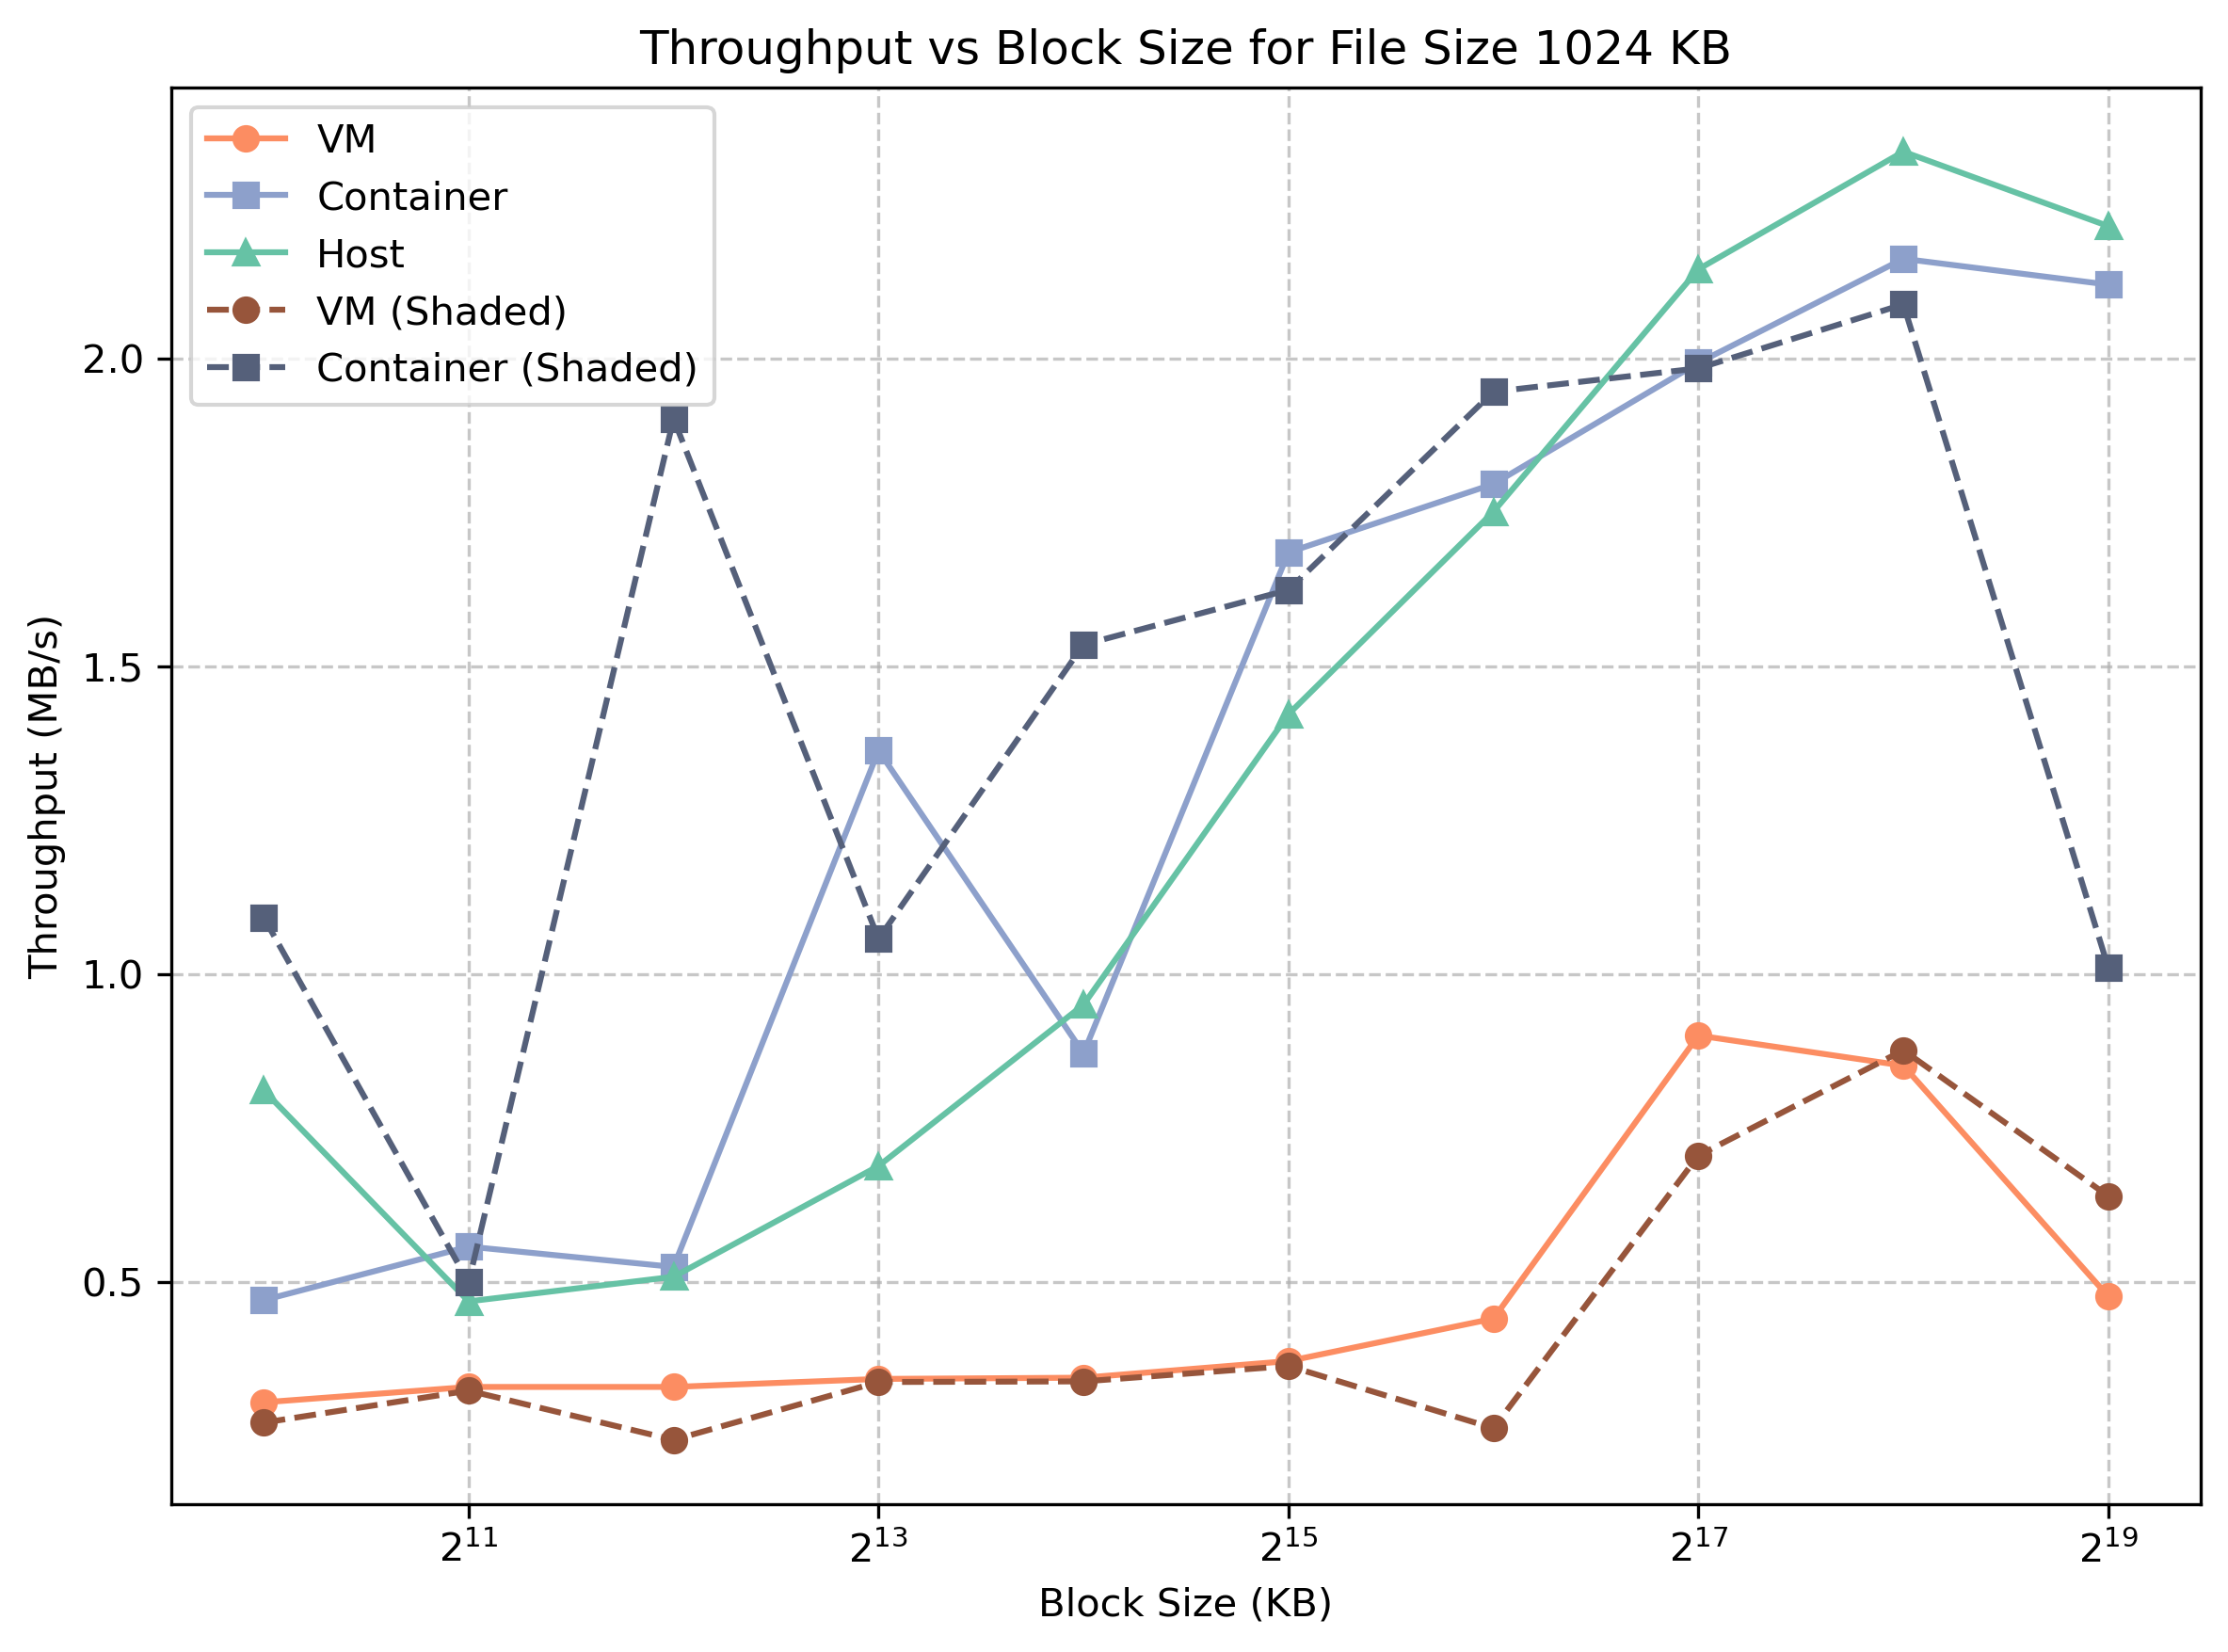
\includegraphics[width=0.8\textwidth]{writer_filesize_1024.png}
  \end{figure}
\end{frame}

\begin{frame}{Iperf}
  % TODO: plot of the bitrate for TCP upload, download, UDP
\end{frame}

\begin{frame}{Conlusion}
  \begin{itemize}
    \item Docker are easier to configure
    \item better performace
  \end{itemize}
\end{frame}

{\setbeamercolor{palette primary}{fg=white, bg=bluscuro}
\begin{frame}[standout]
\thispagestyle{empty}
  {\LARGE Thank You!}
\end{frame}
}



\end{document}
